\documentclass[a4paper,10pt,twoside]{article}
\pdfoutput=1 

\usepackage{amssymb,amsmath}       % Equations
\usepackage{array}
\usepackage{bm}                    % Bold math symbols
\usepackage{epsfig}
\usepackage{float}
\usepackage{graphicx,color,psfrag} % Graphics, Figures
\usepackage{tikz}
\usepackage{multirow}              % For Tables
\usepackage{tabularx}              % Tables
\usepackage{wrapfig}
\usepackage[algoruled]{algorithm2e}
\SetStartEndCondition{ }{}{}%
\SetKwProg{Fn}{def}{\string:}{}
\SetKwFunction{Range}{range}%%
\SetKw{KwTo}{in}\SetKwFor{For}{for}{\string:}{}%
\SetKwIF{If}{ElseIf}{Else}{if}{:}{elif}{else:}{}%
\SetKwFor{While}{while}{:}{}%
% \renewcommand{\forcond}{$i$ \KwTo\Range{$n$}}
\AlgoDontDisplayBlockMarkers\SetAlgoNoEnd\SetAlgoNoLine%


%% enumitem 
% \labelindent is defined in both IEEEtrans and
% enumitem. \let\labelindent\relax kind-of disables \labelindent
% defined in IEEEtrans, hence avoiding the name clash.
\let\labelindent\relax
\usepackage[inline]{enumitem}

%% algorithm2e
% \usepackage[plain]{algorithm2e}
% remove line number for one line
% \let\oldnl\nl
% \newcommand{\nonl}{\renewcommand{\nl}{\let\nl\oldnl}}

%% subfigure
\usepackage[caption=false,font=footnotesize]{subfig}
% make references to subfigures appear as \thefigure(\thesubfigure)
\captionsetup[subfigure]{subrefformat=simple,labelformat=simple,listofformat=subsimple}
\renewcommand\thesubfigure{(\alph{subfigure})}

% variables
\newcommand{\mc}[2][]{{\mathcal{#2}_{\textrm{#1}}}}
\newcommand{\q}[1]{\bm{q}_{\textrm{#1}}}
\newcommand{\qd}[1]{\bm{\dot{q}}_{\textrm{#1}}}
\newcommand{\T}[1]{\bm{T}_{\textrm{#1}}}
\newcommand{\x}[1]{\bm{x}_{\textrm{#1}}}
\newcommand{\qvect}{\bm{q}}
\newcommand{\Tvect}{\bm{T}}
\newcommand{\GP}{\mathcal{G}\cap\mathcal{P}}
\newcommand{\cP}{\mathcal{P}}
\newcommand{\cC}{\mathcal{C}}
\newcommand{\cO}{\mathcal{O}}
\newcommand{\bfp}{\mathbf{p}}
\newcommand{\calT}{\mathcal{T}}
\DeclareMathOperator*{\argmin}{arg\,min}
\DeclareMathOperator*{\argmax}{arg\,max}
% acronyms
\newcommand{\ie}{{\textit{i.e.}}}
\newcommand{\etal}{\textit{et~al.}}

% theorem environment
\newtheorem{theorem}{Theorem}
\newtheorem{proof}{Proof}
\newtheorem{lemma}{Lemma}
\newtheorem{proposition}{Proposition}
\newtheorem{corollary}{Corollary}
\newtheorem{remark}{Remark}
% TODO
\newcommand{\TODO}[1]{\noindent {\color{red} \{{\bf To-do:} #1\}}}
% COMMENT
\newcommand{\comment}[1]{}

% change tt font
\renewcommand{\tt}{\fontfamily{cmtt}\selectfont}

% figures path
\graphicspath{{figures/}}

% \overrideIEEEmargins
% set margins
\setlength{\floatsep}{2pt plus 1pt minus 1pt}
\setlength{\textfloatsep}{5pt plus 1pt minus 2pt}

%% TITLE
\title{MAS714-Homework 2}
%% AUTHOR
\author{Pham Tien Hung, Zhang Xu
}

%% DATE
\date{}


%%%%%%%%%%%%%%%%%%%%%%%%%%%%%%%%%%%%%%%%%%%%%%%%%%%%%%%%%%%%%%%%%%%%%%
\begin{document}
\maketitle
\section*{Exercise 1}
\subsection*{a)}
Prove that every tree is a bipartite graph.
\begin{proof}
	We will prove by induction, that is very tree $T(V, E)$ whose
	$|V| = n$ for all $n$ is a bipartite graph. The case $n=2$ is trivially true.

	Assume that this is true for $|V| = n$, we will now prove that it
	is true for every tree $T'$ whose $|V'| = n + 1$. 

	Consider one such tree $T'$ with $|V'| = n + 1$, we select a leaf node $u$
	and remove it from $T'$ creating $T''$. Clearly, $|V''| = n$ and
	therefore $T''$ is now a bipartite graph. Let $L''$ and $R''$ be the
	corresponding bipartite set of the tree $T''$.

	Without loss of generality, assume that the node $u$ connects to
	some node $v$ belonging to $L''$, we construct two new set $L'$
	and $R'$:
	\[
		L' = L''
	\]
	\[
		R' = R'' \cup \{u\}
	\]
	Clearly, this is enough to say that $T'$ is bipartite.	
\end{proof}

\subsection*{b)}
\begin{algorithm}[h]
  \caption{Check for bipartite graph ($G(V, E)$)}
    T = Kruskal($G$) \;
    L, R are bipartite partition of vertices from $T$ \;
    \TODO{Explain this algorithm in detail} \;
    \For{$(u, v)$ in $E$}{
    	\If{both $u, v$ belongs to L or R}{
    		\Return False
    	}
    }
    \Return True
\end{algorithm}

Time complexity: \TODO{}

Kruskal time complexity is $O(m\log m)$
Bipartite partition took $O(n)$ with BFS (categorised using distance 
to the root node).

Last check took $O(m)$

Total $O(m \log m + n + m) = O(m \log m + n)$

\begin{proof}
	\TODO{}
\end{proof}
\section*{Exercise 2}

Assume that $X_L[1...n]$ is sorted with $X_L[1]$ being the smallest member.

\begin{algorithm}[h]
\caption{Find maximum tiling ($X$)}
	Let $x$ be $-\infty$ \;
	Initialize $T = \emptyset$\;
	\While{$X$ is not empty}{
		\eIf {$X_L[0] > x$}{
			Let $x_{stop} = X_L[0]$\;
		}{Let $x_{stop} = x$}
		Let $x_{max} = -\infty$\;
		\While{$X_L[0] \leq x_{stop}$}{
			\If {$X_R[0] > x_{max}$}{
				$x_{max} = X_R[0]$\;
				Select $X[0]$ as the chosen interval $i$\;
			}
			Remove $X[0]$ from $X$\;
		}
		Add the selected interval $i$ to $T$\;
		% Let $O$ be the set of interval such that $X_L[i] \leq x$\;
		% \If {$O == \emptyset$}{
		% 	Let $O$ be the set of interval such that $X_L[i] == X_L[0]$\;
		% }
		% Let $X = X \setminus O$\;
		% Sort $O$ according to the right end point\;
		% Let $y = \argmax_{i \in O} i_R$\;
		% Let $T = T\cup\{y\}$\;
		% Let $x = y_R$\;
	}
	\Return $T$\;
\end{algorithm}
Running time $O(n)$.

\section*{Exercise 3}

\subsection*{a}
Not all Minimum Bottleneck Tree (MBT) is a MST. Here is an counter example:

\begin{figure}[h]
	\centering
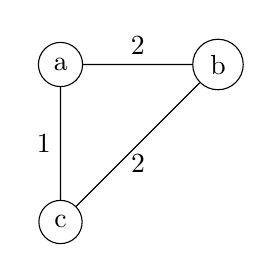
\begin{tikzpicture}
	\path 	(0, 2) node[circle, radius=2.5pt, draw] (a) {a}
			(2, 2) node[circle, radius=2.5pt, draw] (b) {b}
			(0, 0) node[circle, radius=2.5pt, draw] (c) {c};
	\draw (a) 
				-- node[above] {2} (b) 
				-- node[below] {2} (c) 
				-- node[left] {1} (a);
\end{tikzpicture}
	\label{fig:figure1}
\end{figure}
The tree containing two edges $(a, b), (b, c)$ is an MBT but is clearly
not a MST.

\subsection*{b}
We will show that given an undirect graph $G$ with distinct edge
cost, if $T$ is $G$'s minimum spanning
tree (MST) then it is also a minimum-bottleneck tree (MBT) of $G$.
\begin{proof}
	We will prove by contradition. That is, let $T$ be an MST of $G$,
	there must exist a spanning tree $T'$ whose maximum edge cost
	being smaller than the maximum edge cost of $T$.
	Let $e_i$ and $e'_i$ denote the edges of $T$ and $T'$ respectively.
	This means
	\[
		\max_i{e'_i} < \max_i{e_i}.
	\]

	Now, we modify the tree $T'$ to by iteratively
	loop through each edge $e'_i$ and check if it is a safe edge crossing
	the corresponding cut $(S'_i, V\setminus S'_i)$. If $e'_i$ is a safe
	edge, then it is left unchanged else it is replaced with the safe edge
	crossing the cut $(S'_i, V\setminus S'_i)$.
	After any iteration $j$, the following hold:
	\begin{enumerate}
		\item The modified tree remains a spanning tree.
		\item All modifed edges $e'_1, ..., e'_j$ are safe edges.
	\end{enumerate}

	Both implies that after the operation, the modifed tree is an MST.
	Denoting the new tree $T''$, since the set of safe edges form the unique
	minimum spanning tree under the condition of distinct edge cost, clealy
	$T''$ is the unique MST of $G$. Therefore, $T'' = T'$.

	In the operation, we only replace an edge $e'_j$ if it is not a safe edge,
	this means cost of all edges can only decrease. This means:
	\[
		e''_j \leq e'_j, \forall j
	\]
	which implies
	\[
	\begin{aligned}
		\max_i e''_i &\leq \max_i e'_i \\
					 &< \max_i e_i\\
					 &< \max_i e''_i\\,
	\end{aligned}
	\]
	which is clearly a contradition.
\end{proof}
\section*{Exercise 4}
\subsection*{a}
Do DFS on the spanning tree, find the path between $u, v$.
Check if all the edges connecting this path has weight lower than $c$.
If true, then $T$ is no longer the MST, else it is.

Complexity $O(n)$.

\subsection*{b}
Just go over each edge and fix them individually.


\section*{Exercise 5}
\subsection*{a}

Take log of each edge weight then do shortest path.
\end{document}
